
\documentclass[12pt,a4paper]{article}

% Pacotes básicos
\usepackage[utf8]{inputenc}
\usepackage[T1]{fontenc}
\usepackage[brazil]{babel}
\usepackage{graphicx}
\usepackage{float}
\usepackage{amsmath, amssymb}
\usepackage{hyperref}
\usepackage{caption}
\usepackage{cite}
\usepackage{listings} % para formatar blocos de código
\usepackage{enumitem} % para controlar listas
\usepackage{xcolor}   % necessário para cores no listings

% Configurações do listings
\lstset{
  language=Python,
  basicstyle=\ttfamily\small,
  numbers=left,
  numberstyle=\tiny,
  frame=single,
  breaklines=true,
  keywordstyle=\color{blue}\bfseries,
  stringstyle=\color{red},
  commentstyle=\color{green!60!black}\itshape,
  showstringspaces=false
}

\graphicspath{{./}{../}{../../}{../../plots/}{../../plots/img/}}

% \title{Relatório do Projeto de Grafos e Algoritmos de Busca}
% \author{
% Áquila Oliveira Souza | 2021019327 \\ 
% Felippe Veloso Marinho | 2021072260 \\ 
% Jefferson Pereira de Souza | 2022099049
% }
% \date{\today}

\begin{document}

% ==============================
% CAPA
% ==============================
\begin{titlepage}
    \centering
    {\Large \textbf{Universidade Federal de Minas Gerais}}\\[0.3cm]
    {\large Engenharia de Sistemas}\\[2cm]
    
    {\Huge \textbf{Relatório do Projeto de Grafos e Algoritmos de Busca}}\\[1.5cm]
    
    \textbf{Fundamentos de Inteligência Artificial}\\[0.5cm]
    \textbf{Professores:} Cristiano Castro e João Pedro Campos\\[1.5cm]
    
    \begin{flushleft}
        \textbf{Alunos:}\\
        Áquila Oliveira Souza --- 2021019327\\
        Arthur Jorge --- 2022055718\\
        Felippe Veloso Marinho --- 2021072260\\
        Jefferson Pereira de Souza --- 2022099049\\
        Josoé Santos Queiroz --- 2019026982
    \end{flushleft}
    
    \vfill
    {\large Belo Horizonte, MG}\\
    {\large \today}
\end{titlepage}

\clearpage
\tableofcontents
\clearpage

% ==============================
% INTRODUÇÃO
% ==============================
\section{Introdução}
Este relatório tem como objetivo apresentar a solução para o clássico \textit{Problema da Ponte e da Tocha}, um quebra-cabeça que serve como excelente caso de estudo para a aplicação de algoritmos de busca e a modelagem de problemas em grafos. O problema consiste em mover um grupo de pessoas de um lado para o outro de uma ponte sob condições específicas, minimizando o tempo total da travessia.

Para resolver este problema, o projeto foi modelado formalmente como um problema de busca em espaço de estados, onde cada estado representa uma configuração possível das pessoas e da tocha. As transições entre estados são as ações de travessia. Essa abordagem permite construir um grafo completo de estados, ideal para testar e comparar diferentes algoritmos.

Ao longo deste documento, detalharemos a modelagem do problema, as rotinas de busca implementadas — incluindo Busca em Largura (BFS), Busca em Profundidade (DFS) e o algoritmo A* — e, por fim, compararemos seus resultados para determinar a eficiência de cada método na busca pela solução ótima.

% \cite{cormen}.

\section{Modelagem do Problema em Forma de Grafo}
O problema da \textit{Ponte e da Tocha} foi modelado como um problema de busca em espaço de estados e também como um CSP (\textit{Constraint Satisfaction Problem}). Essa abordagem permite tanto a análise formal do problema em termos de grafos, como também a aplicação de algoritmos de busca clássicos para encontrar soluções ótimas. 

A seguir, a modelagem será descrita em camadas: definição de estados, ações, função sucessora e custos.

% \subsection{Variáveis}
% Para modelar o problema da ponte com $N$ pessoas como um COP, definimos um conjunto de variáveis de decisão. A variável principal é o tempo de travessia de cada pessoa, e as variáveis auxiliares nos ajudarão a definir a sequência de movimentos.

% \begin{itemize}
%     \item $t_i$: Variável que representa o tempo de travessia para a pessoa $i \in \{1, \dots, N\}$.
%     \item $m_{i,j,k}$: Variável binária, onde $m_{i,j,k} = 1$ se as pessoas $i$ e $j$ atravessam a ponte juntas no passo $k$ (ida ou volta). Se apenas a pessoa $i$ atravessar, usamos $m_{i,0,k}$.
%     \item $s_{i,k}$: Variável binária, onde $s_{i,k} = 1$ se a pessoa $i$ estiver no lado de partida (origem) após o passo $k$.
%     \item $p_k$: Variável binária, onde $p_k=1$ se o passo $k$ é uma travessia de ida e $p_k=0$ se é uma travessia de volta.
% \end{itemize}

% \subsection{Domínio das Variáveis}
% \begin{itemize}
%     \item $t_i \in \{T_1, T_2, \dots, T_N\}$, onde $T_i$ é o tempo individual da pessoa $i$.
%     \item $m_{i,j,k} \in \{0, 1\}$.
%     \item $s_{i,k} \in \{0, 1\}$.
%     \item $p_k \in \{0, 1\}$.
% \end{itemize}

% \subsection{Função Objetivo}
% Nosso objetivo é minimizar o tempo total da travessia, que é a soma dos tempos de cada movimento.

% \[
% \min \sum_{k=1}^{K} \left( \sum_{i=1}^{N} \sum_{j=0}^{N} m_{i,j,k} \cdot \max(T_i, T_j) \right)
% \]

% Onde $T_0$ é o tempo de uma "pessoa imaginária" com tempo 0, para os casos de travessia única ($j=0$).
% O número de passos $K$ pode ser estimado, mas não é fixo a priori.

% \subsection{Restrições}
% \subsubsection{Restrições de Movimento e Posição}
% \begin{enumerate}
%     \item \textbf{Apenas uma ação por passo:}
%     \[
%     \sum_{i=1}^{N} \sum_{j=i}^{N} m_{i,j,k} + \sum_{i=1}^{N} m_{i,0,k} = 1 \quad \forall k
%     \]
%     \item \textbf{Consistência da Posição:}
%     \[
%     s_{i,k} = s_{i,k-1} + (p_k \cdot (\sum_{j=1}^{N} m_{i,j,k})) - ((1-p_k) \cdot (\sum_{j=1}^{N} m_{i,j,k})) \quad \forall i,k
%     \]
%     \item \textbf{Restrição da Tocha:}
%     \[
%     p_k = 1 - p_{k-1} \quad \forall k > 1
%     \]
% \end{enumerate}

\subsection{Estados}
Seguindo a descrição do enunciado e visualizando a implementação em código, o estado do problema é representado por um array binário, que fornece uma representação compacta e eficiente.
\[
S = [p_1, p_2, p_3, p_4, t]
\]

Onde:
\begin{itemize}
    \item $p_i \in \{0, 1\}$ indica a posição da pessoa $i$ (A, B, C, D, respectivamente), onde $0$ representa o lado inicial (esquerdo) e $1$ representa o lado final (direito);
    \item $t \in \{0, 1\}$ indica a posição da tocha, onde $0$ representa o lado inicial e $1$ o lado final.
\end{itemize}

Assim, temos:
\begin{itemize}
    \item \textbf{Estado inicial}: $[0, 0, 0, 0, 0]$ (todas as pessoas e a tocha no lado inicial);
    \item \textbf{Estado objetivo}: $[1, 1, 1, 1, 1]$ (todas as pessoas e a tocha no lado final).
\end{itemize}

O lado final da ponte é implicitamente definido como o complemento do lado inicial.

\subsection{Ações e Função Sucessora}
Cada ação corresponde ao movimento de uma ou duas pessoas através da ponte, levando sempre a tocha consigo. A função sucessora gera todos os estados possíveis a partir de um estado atual, respeitando as regras do problema.

\begin{itemize}
    \item Se a tocha está no lado inicial ($t = 0$): escolher 1 ou 2 pessoas que estão no lado inicial ($p_i = 0$) para atravessar para o lado final;
    \item Se a tocha está no lado final ($t = 1$): escolher 1 ou 2 pessoas que estão no lado final ($p_i = 1$) para retornar ao lado inicial.
\end{itemize}

O custo de cada ação é definido como o tempo da travessia, que corresponde ao tempo da pessoa mais lenta entre as selecionadas.

\subsection{Exemplos Ilustrativos de Caminhos}
Para uma melhor clareza e visualização nos diagramas de grafo, os estados são representados utilizando a notação textual original, com o conjunto de pessoas no lado inicial e a posição da tocha. Por exemplo, o estado $[0, 0, 0, 0, 0]$ é visualizado como `({A, B, C, D}, início)`, e o estado $[1, 1, 1, 1, 1]$ como `({}, final)`. Esta representação é mais intuitiva para o entendimento humano, embora a implementação do código utilize a representação binária mais eficiente.

A Figura \ref{fig:optimal_path} mostra o caminho ótimo com cinco movimentos e custo total de 17 minutos.

\begin{figure}[H]
    \centering
    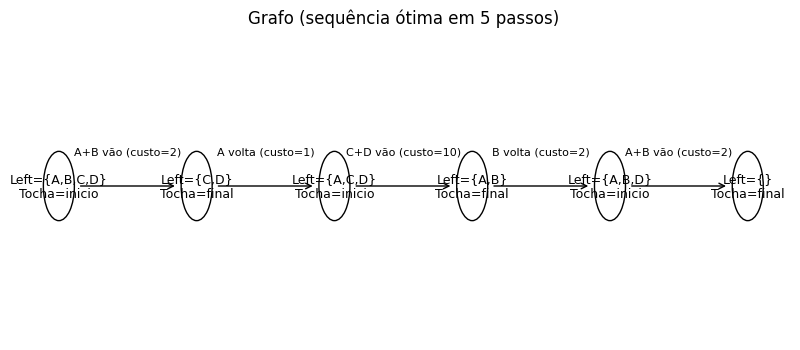
\includegraphics[width=0.8\linewidth]{optimal_path.png}
    \caption{Caminho ótimo de travessia em cinco passos (custo total de 17 minutos).}
    \label{fig:optimal_path}
\end{figure}

A Figura \ref{fig:ramification} mostra um exemplo de ramificação do grafo de estados.

\begin{figure}[H]
    \centering
    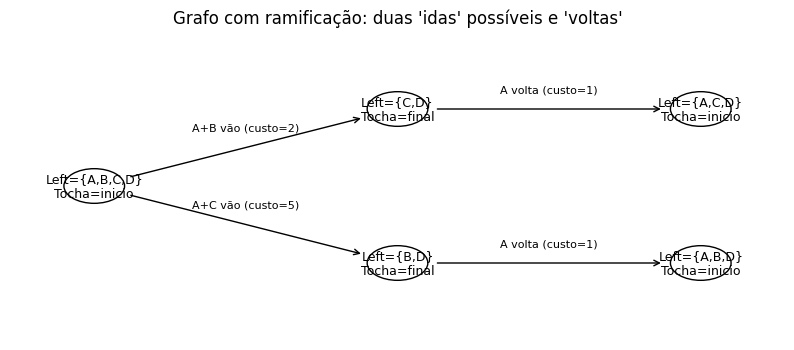
\includegraphics[width=0.8\linewidth]{ramification.png}
    \caption{Ramificação do grafo de estados com duas escolhas iniciais.}
    \label{fig:ramification}
\end{figure}

Por fim, a figura \ref{fig:full_graph} apresenta o grafo completo do problema com 4 pessoas, ilustrando todos os estados possíveis e transições. As legendas de cada ponto no grafo mostram a representação binária de cada estado. Essa visualização é crucial para entender a estrutura do espaço de estados e a complexidade do problema.

\begin{figure}[H]
    \centering
    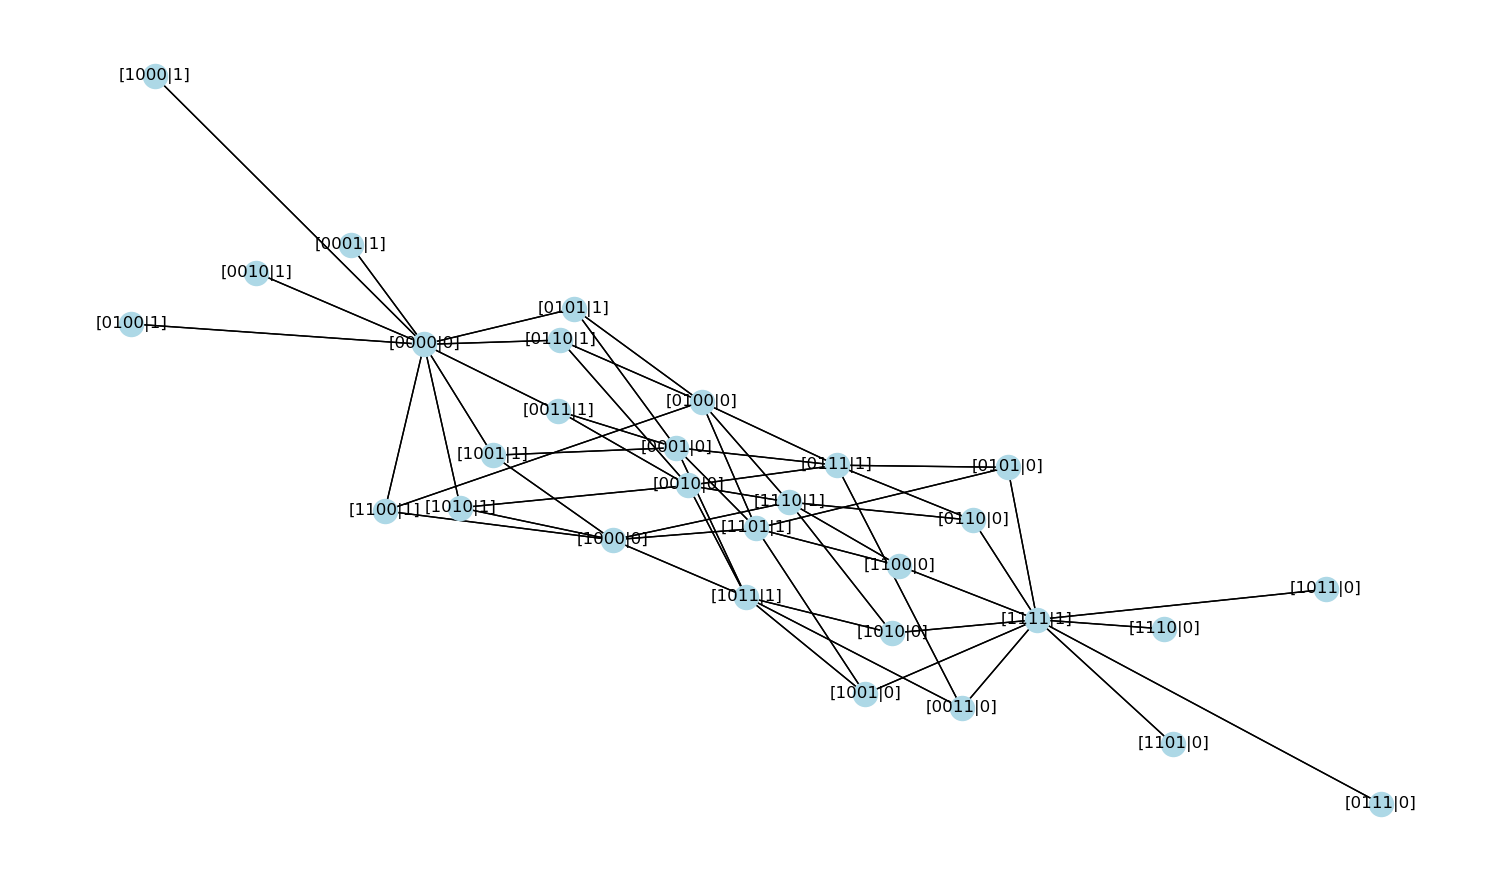
\includegraphics[width=0.8\linewidth]{graph_complete_labels.png}
    \caption{Grafo completo do problema com 4 pessoas, ilustrando todos os estados possíveis e transições.}
    \label{fig:full_graph}
\end{figure}

\subsection{Definição Formal do Grafo}
De forma resumida:
\begin{itemize}
\item \textbf{Vértices}: cada vértice corresponde a um estado $S = [p_1, p_2, p_3, p_4, t]$;
\item \textbf{Arestas}: cada aresta representa uma ação válida (ida ou volta de 1 ou 2 pessoas), com custo associado ao tempo da travessia;
\item \textbf{Justificativa}: essa modelagem é natural porque o espaço de estados é finito e discreto, permitindo a aplicação direta de algoritmos de busca como BFS e DFS.
\end{itemize}

\section{Rotinas Desenvolvidas}

\subsection{Estrutura geral do código}

Para permitir a escalabilidade do problema, os tempos foram definidos da seguinte forma:

\begin{lstlisting}
TIMES = [1, 2, 5, 10] + [fib_n(i)*10 for i in range(4, N)]
\end{lstlisting}

Dessa maneira, para o cenário básico, se o número de pessoas $N$ for igual a 4, a lista
\texttt{[fib\_n(i)*10 for i in range(4, N)]} se torna uma lista vazia, mantendo os tempos clássicos do enunciado.

Para verificar casos maiores, ao aumentar $N$, a lista se expande conforme a função \texttt{fib\_n(n)}, que calcula o $n$-ésimo número de Fibonacci.

Por exemplo, se $N = 6$:
\begin{itemize}
    \item $fib_n(4) = 3 \Rightarrow 3 \times 10 = 30$
    \item $fib_n(5) = 5 \Rightarrow 5 \times 10 = 50$
\end{itemize}

Assim, a nova lista de tempos será:
\[
TIMES = [1, 2, 5, 10, 30, 50]
\]

\subsection{Funções principais}
\begin{itemize}
    \item \textbf{\texttt{cost(movers)}}: Calcula o custo de uma travessia (tempo da pessoa mais lenta).
    \item \textbf{\texttt{successors(state)}}: Gera todos os estados sucessores válidos a partir de um estado.
    \item \textbf{\texttt{astar\_heuristic()}}: estima o custo mínimo de tempo necessário para que todas as pessoas no lado esquerdo da ponte cheguem ao lado direito.
    \begin{itemize}
        \item A função é dividida em dois casos, dependendo da posição da tocha, para fornecer uma estimativa precisa e otimista:
        \item \textbf{Tocha no lado esquerdo:} O custo estimado é a soma do tempo das duas pessoas mais lentas que restam, pois elas definem o custo mínimo de travessia para o restante do grupo. Se resta apenas uma pessoa, o custo é o tempo dela.
        \item \textbf{Tocha no lado direito:} O custo estimado é o tempo da pessoa mais rápida que está no lado direito, pois ela é a candidata ideal para retornar a tocha.
    \end{itemize}
    \item \textbf{\texttt{bfs() / dfs() / astar()}}: Implementam os algoritmos de busca clássicos empregados na resolução do problema, descritos a seguir de forma geral.
\end{itemize}

Os três algoritmos utilizados compartilham a mesma estrutura conceitual básica: a exploração sistemática do espaço de estados do problema, a partir de um estado inicial, até alcançar o estado objetivo. O que os diferencia é a forma como cada um escolhe qual estado expandir a cada iteração.

\subsubsection{Busca em Largura (BFS)} 
A \textit{Breadth-First Search} realiza uma busca em camadas, explorando primeiro todos os estados alcançáveis com um número mínimo de passos antes de avançar para níveis mais profundos. 
É garantido que a BFS encontra a solução ótima quando o custo de cada transição é uniforme. No contexto do problema da ponte, isso equivale a encontrar a sequência de travessias com o menor número de movimentos, ainda que não necessariamente com o menor tempo total.

\subsubsection{Busca em Profundidade (DFS)} 
A \textit{Depth-First Search} adota uma abordagem recursiva ou baseada em pilha, explorando o caminho atual até o limite antes de retroceder. 
Embora possa ser mais eficiente em memória, a DFS não garante a optimalidade da solução, e em alguns casos pode se perder em ramos muito profundos ou redundantes. No entanto, é útil para compreender a estrutura do grafo de estados e verificar a conectividade do espaço de busca.

\subsubsection{Busca A* (A Estrela)} 
O algoritmo \textit{A*} combina os princípios da busca em largura com uma função heurística $h(n)$ que estima o custo restante até o objetivo. 
Ele utiliza uma função de avaliação $f(n) = g(n) + h(n)$, onde $g(n)$ é o custo acumulado até o nó atual e $h(n)$ é a estimativa do custo restante. 
Essa combinação permite que o A* explore o espaço de busca de maneira informada, priorizando os caminhos mais promissores e garantindo a solução ótima desde que a heurística seja admissível (isto é, nunca superestime o custo real).

\section{Algoritmos de Busca Estudados}
Nesta seção, são detalhados os algoritmos de busca implementados no projeto: \textbf{Busca em Largura (BFS)}, \textbf{Busca em Profundidade (DFS)}, \textbf{Dijkstra} e \textbf{A*}. 
Cada um deles foi adaptado para operar sobre a estrutura de grafo que modela os estados possíveis do problema da Ponte e da Tocha, buscando o caminho que leva do estado inicial ao estado objetivo com o menor custo total.

\subsection{Busca em Largura (BFS)}
A \textit{Breadth-First Search} é um dos algoritmos mais fundamentais da teoria dos grafos. Sua lógica baseia-se em percorrer o grafo em \textit{camadas}, garantindo que todos os vértices a uma mesma distância do ponto de origem sejam explorados antes de prosseguir para níveis mais profundos. 
No código implementado, a BFS utiliza uma \textbf{fila} (\texttt{deque}) para armazenar os vértices a serem visitados e dicionários para registrar:
\begin{itemize}
    \item as distâncias mínimas até cada vértice (\texttt{dist});
    \item e o vértice predecessor em relação a cada nó (\texttt{predecessor}), utilizado posteriormente na reconstrução do caminho.
\end{itemize}

\begin{lstlisting}[caption={Trecho simplificado da função BFS.}]
def bfs(graph, start):
    dist = {vertex: float("inf") for vertex in graph.graph}
    predecessor = {vertex: None for vertex in graph.graph}
    dist[start] = 0
    queue = deque([start])
    
    while queue:
        current_vertex = queue.popleft()
        for edge in graph.graph[current_vertex]:
            neighbor = edge.v
            if dist[neighbor] == float("inf"):
                dist[neighbor] = dist[current_vertex] + 1
                predecessor[neighbor] = current_vertex
                queue.append(neighbor)
    return dist, predecessor
\end{lstlisting}

A BFS garante a descoberta do caminho com o menor número de passos, mas não necessariamente com o menor custo acumulado. Por isso, seu uso neste problema serve como referência estrutural, e não como método ótimo em termos de tempo total de travessia.

\subsection{Busca em Profundidade (DFS)}
A \textit{Depth-First Search} é um algoritmo que explora o grafo de maneira recursiva ou iterativa, aprofundando-se em um caminho até que não haja mais vértices não visitados. Em seguida, realiza o retrocesso (\textit{backtracking}) para explorar outras alternativas.

A implementação utiliza uma \textbf{pilha} para controlar os vértices a visitar e um conjunto \texttt{visited} para evitar repetições.

\begin{lstlisting}[caption={Trecho simplificado da função DFS.}]
def dfs(graph, start):
    visited = set()
    stack = [start]
    predecessor = {start: None}
    while stack:
        vertex = stack.pop()
        if vertex not in visited:
            visited.add(vertex)
            for edge in graph.get(vertex, []):
                neighbor = edge.v
                if neighbor not in visited:
                    stack.append(neighbor)
                    predecessor[neighbor] = vertex
    return predecessor
\end{lstlisting}

Embora não garanta o caminho ótimo, o DFS é útil para compreender a estrutura de conectividade do grafo e para verificar se todos os estados são alcançáveis a partir de uma dada configuração inicial. Sua vantagem está na baixa utilização de memória, uma vez que armazena apenas o caminho atual.

\subsection{Algoritmo de Dijkstra}
O algoritmo de Dijkstra é um método clássico para encontrar o caminho de menor custo entre um nó de origem e todos os outros vértices de um grafo ponderado com pesos não negativos. 
Diferentemente da BFS, que assume custos unitários, Dijkstra considera explicitamente os pesos das arestas --- no caso do problema estudado, o tempo de travessia entre estados.

A implementação utiliza uma \textbf{fila de prioridade} (\texttt{heapq}) para sempre expandir o vértice com a menor distância acumulada (\( g(n) \)).

\begin{lstlisting}[caption={Trecho da função Dijkstra.}]
def dijkstra(graph, start):
    dist = {vertex: float("inf") for vertex in graph}
    predecessor = {vertex: None for vertex in graph}
    dist[start] = 0
    pq = [(0, start)]

    while pq:
        current_dist, current_vertex = heappop(pq)
        for edge in graph[current_vertex]:
            neighbor, weight = edge.v, edge.w
            distance = current_dist + weight
            if distance < dist[neighbor]:
                dist[neighbor] = distance
                predecessor[neighbor] = current_vertex
                heappush(pq, (distance, neighbor))
    return dist, predecessor
\end{lstlisting}

O algoritmo retorna, portanto, tanto o custo mínimo de cada vértice a partir da origem quanto o dicionário de predecessores, o que permite reconstruir o caminho ótimo até o destino. 
No contexto da Ponte e da Tocha, ele representa uma versão determinística e exata para a minimização do tempo total de travessia, considerando pesos reais associados a cada transição.

\subsection{Algoritmo A* (A Estrela)}
O algoritmo A* combina os princípios do Dijkstra com o uso de uma \textbf{função heurística} \( h(n) \), que estima o custo restante até o objetivo. 
Ele avalia cada estado por meio da função:
\[
f(n) = g(n) + h(n)
\]
onde:
\begin{itemize}
    \item \( g(n) \) é o custo acumulado desde o início até o nó atual;
    \item \( h(n) \) é a estimativa do custo restante até o estado objetivo.
\end{itemize}

No código, o conjunto de nós abertos (\texttt{open\_set}) é gerenciado como uma fila de prioridade. A cada iteração, o nó com o menor valor de \( f(n) \) é expandido.

\begin{lstlisting}[caption={Trecho da função A*.}]
def a_star(graph, start, goal, heuristic):
    from heapq import heappop, heappush
    open_set = []
    heappush(open_set, (heuristic(start), 0, start))
    came_from = {}
    g_score = {v: float("inf") for v in graph}
    g_score[start] = 0
    
    while open_set:
        _, g, current = heappop(open_set)
        if current == goal:
            return reconstruct_path(came_from, start, goal)
        for edge in graph[current]:
            neighbor, weight = edge.v, edge.w
            tentative_g = g + weight
            if tentative_g < g_score[neighbor]:
                came_from[neighbor] = current
                g_score[neighbor] = tentative_g
                f_score = tentative_g + heuristic(neighbor)
                heappush(open_set, (f_score, tentative_g, neighbor))
    return []
\end{lstlisting}

O desempenho do A* depende fortemente da escolha da heurística. 
Se \( h(n) \) for \textit{admissível} (isto é, nunca superestimar o custo real até o objetivo), o A* garante não a optimalidade da solução, mas tende a explorar menos nós que o Dijkstra, reduzindo significativamente o tempo de execução.

\subsection{Comparativo geral}
A Tabela \ref{tab:comparativo} resume as principais características e diferenças entre os algoritmos implementados.

\begin{table}[H]
\centering
\caption{Comparativo geral entre os algoritmos de busca (h = heurística).}
\label{tab:comparativo}
\begin{tabular}{|l|c|c|c|c|}
\hline
\textbf{Algoritmo} & \textbf{EDs} & \textbf{Custos?} & \textbf{Optimalidade} & \textbf{Memória}\\
\hline
BFS & Queue & Não & Sim (para custos iguais) & Moderada \\
\hline
DFS & Stack & Não & Não & Baixa \\
\hline
Dijkstra & Queue & Sim & Sim & Alta \\
\hline
A* & Queue + h & Sim & Sim (se h ok) & Variável \\
\hline
\end{tabular}
\end{table}

A escolha do algoritmo ideal depende da natureza do problema e da disponibilidade de informações adicionais. 
Para o caso da Ponte e da Tocha, o A* demonstrou ser o método mais eficiente em termos de custo computacional e qualidade da solução, quando utilizada uma heurística adequada à estrutura do problema.

\section{Comparação e Discussão dos Resultados}
% Comparar os algoritmos aplicados para solucionar o puzzle.
% \begin{itemize}
%     \item Critérios de comparação (tempo de execução, número de passos, consumo de memória, etc.);
%     \item Tabelas e gráficos com resultados;
%     \item Discussão dos pontos fortes e fracos de cada abordagem.
% \end{itemize}

Vimos anteriormente que os algoritmos BFS e DFS possuem complexidade de tempo $O(n)$, enquanto Dijkstra e A* possuem complexidade $O(n \log n)$. Ao realizar a análise experimental, observa-se que Dijkstra apresenta o maior custo entre os algoritmos, enquanto o custo do A* é o menor. Isso ocorre porque a heurística escolhida foi adequada, reduzindo significativamente a quantidade de nós explorados no grafo.

O a figura \ref{fig:fig_graph_comparsion} mostra a comparação das soluções encontradas pelos algoritmos para o problema com 4 pessoas. As cores representam os diferentes algoritmos: BFS (vermelho), DFS (verde), Dijkstra (azul) e A* (laranja). Neste pode-se notar uma pequena diferença entre as soluções encontradas por Dijkstra e A*, ambas próximas do ótimo, enquanto BFS e DFS resultam em soluções com custo consideravelmente maior.

\begin{figure}[H]
    \centering
    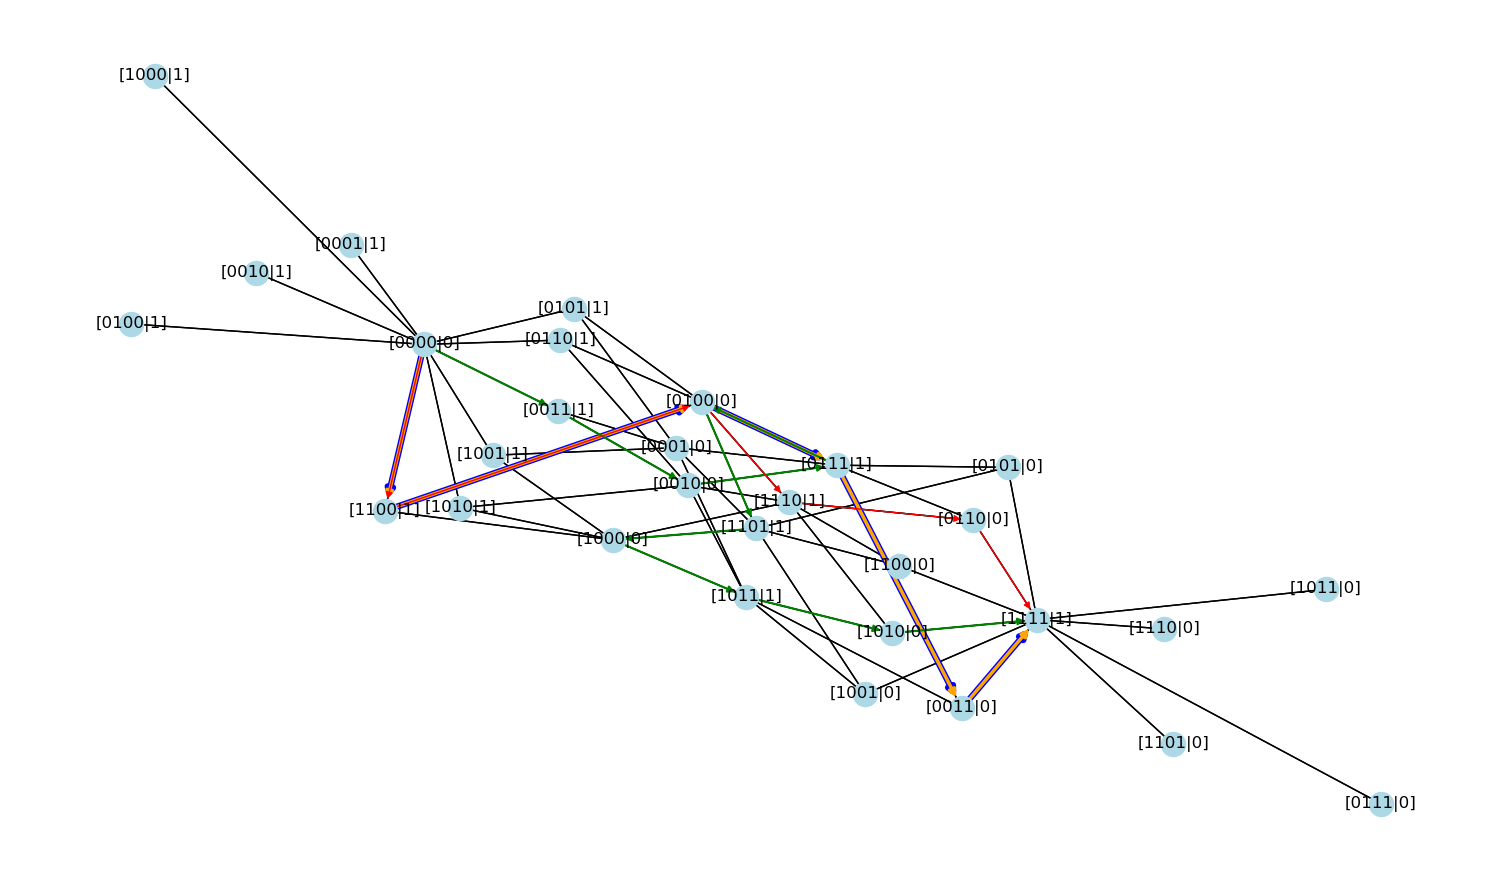
\includegraphics[width=0.8\linewidth]{graph_comparsion_complete_labels.png}
    \caption{Comparação das soluções encontradas pelos algoritmos para o problema com 4 pessoas.}
    \label{fig:fig_graph_comparsion}
    \hspace{\fill}
\end{figure}


\begin{figure}[H]
    \centering
    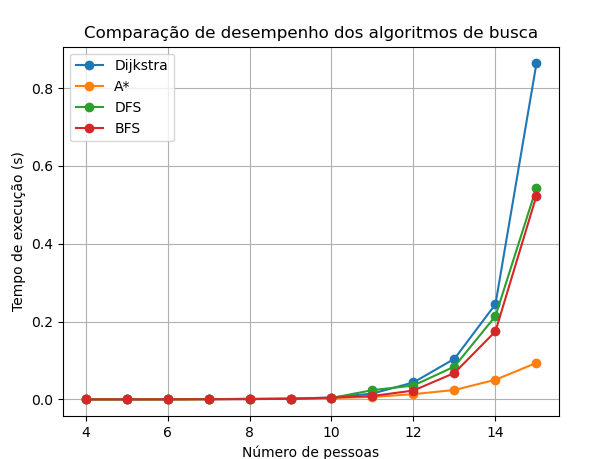
\includegraphics[width=0.8\linewidth]{execution_time.png}
    \caption{Tempo de execução em função do número de pessoas.}
    \label{fig:execution_time}
\end{figure}

No grafico abaixo é possivel perceber que o A* é muito eficiente em eliminar nós desnecessarios, enquanto o DFS visita a maior quantidade, chegando a um milhão de nós visitados em um problema com 15 pessoas.

\begin{figure}[H]
    \centering
    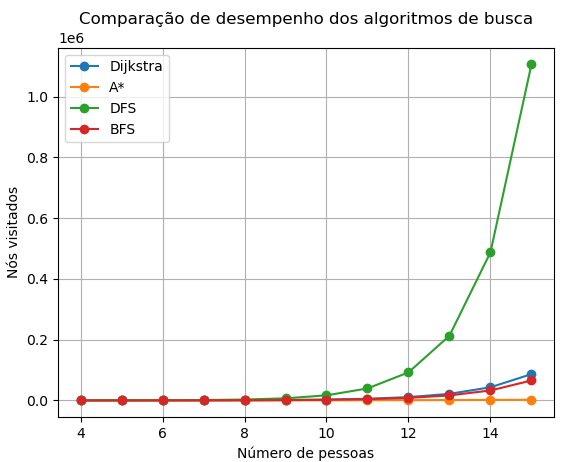
\includegraphics[width=0.8\linewidth]{node_visited.png}
    \caption{Número de nós visitados em função da quantidade de pessoas.}
    \label{fig:node_visited}
\end{figure}

É importante notar também que o algoritmo BFS não garante solução ótima. Isso ocorre pois dois estados obtidos a partir do mesmo estado são explorados na mesma iteração, independentemente do seu custo. Assim, um caminho ótimo que passa por muitos estados de baixo custo pode ser explorado somente após um caminho não ótimo com poucos estados de maior custo.  
Por outro lado, os algoritmos Dijkstra e A* retornam soluções com bastante muito reduzido em relação ao BFS e DFS, que não consideram o custo das arestas. Contudo, o A* se destaca por explorar menos nós que o Dijkstra, usando uma heurística para sempre buscar soluções mais próximas do ótimo com menos custo computacional.
\section{Conclusão}

Este trabalho demonstrou a eficácia da modelagem do problema da Ponte e da Tocha como um problema de busca em espaço de estados, permitindo a aplicação e comparação sistemática de algoritmos clássicos de busca. A análise experimental evidenciou diferenças significativas entre eles em termos de eficiência, consumo de memória e garantia de optimalidade.  

Foi possível observar que BFS e DFS, apesar de simples, apresentam limitações quanto à optimalidade quando os custos variam. Dijkstra garante soluções ótimas considerando custos, porém com maior custo computacional. O algoritmo A*, com uma heurística adequada, mostrou ser o mais eficiente, reduzindo bastante o número de nós explorados e o tempo de execução.  

Os principais aprendizados incluem a importância de uma modelagem eficiente, a escolha adequada de estruturas de dados e o papel determinante de heurísticas na performance de algoritmos informados.  

Como melhorias futuras, recomenda-se explorar heurísticas mais sofisticadas para o A*, investigar abordagens híbridas ou baseadas em aprendizado de máquina para estimativas de custo, e testar a modelagem em versões mais complexas do problema, incluindo restrições adicionais, visando ampliar a aplicabilidade e otimização das soluções.

% \section*{Referências}
\clearpage
\addcontentsline{toc}{section}{Referências}
\bibliographystyle{plain}
\bibliography{references}

\end{document}
